\chapter{Specification for the report}
    To ensure a good outline of the project is given specification needs to be provided for various parts of the system to later on lead the design, implementation and testing of the environment. The following sections break down the system into its biggest parts and give a set of requirements as guidelines.

    \section{The simulation environment}
      The robot environment will be the center of emulating the environment. It will be responsible for housing the Robot Operating System server with maps, odometry for robots and mapping the robots inside a map so that they will be able to move around and accept commands from outside sources i.e. the GUI and transfer these commands into robot movement and task allocation. Below is the outlined specification for the environment.

      \begin{itemize}
        \item \textbf{SE1}: ROS based simulation environment.
        \item \textbf{SE2}: An environment that allows simulation of a robot on a 2-D plane with the map received from project supervisor.
        \item \textbf{SE3}: Accepting commands from outside sources that guide the robot e.g. Go to room 1.
        \item \textbf{SE4}: Responding to commands about robots position and whether it reached its goal.
        \item \textbf{SE5}: An ability for the robot to realize which rooms are closest to it.
        \item \textbf{SE6}: Robot is able to find its own way inside the map to the goal.
        \item \textbf{SE7}: Allow for more than one robot in a single simulation.
        \item \textbf{SE8}: Robot is fully aware of another robots presence.
        \item \textbf{SE9}: Robot is able to avoid collisions with other robots.
        \item \textbf{SE10}: The environment can accept various maps and robots can adapt to these.
        \item \textbf{SE11}:  (Optional) Simulation minimizes the use of system resources.
      \end{itemize}

    \section{Graphical User Interface}
      The Graphical User Interface is a crucial aspect to how the task distribution will be managed. Whether it is click and go or hot keyed commands is a question that will be crucial here. The human factor needs to be taken into account as basis for testing but having a user interface that doesn't allow comfortable work will only result in slowing down the human factor and making the results biased towards the robots working by themselves. Below is the outlined specification for the GUI.
      
        \begin{itemize}
          \item \textbf{UI1}: Interface should provide an approximated view of the simulation.
          \item \textbf{UI2}: Interface provides options for users to select rooms that robots go to.
          \item \textbf{UI3}: Users are able to select robots that they want to send goals for.
          \item \textbf{UI4}: User has the option of identifying the treasure, taking the picture and moving on.
          \item \textbf{UI5}: Upon receiving the picture user has the option to take the treasure.
          \item \textbf{UI6}: Interface contains the map with an outline of rooms.
          \item \textbf{UI7}: Interface updates robots positions on the map based on where they are in the simulation.
          \item \textbf{UI8}: Interface accepts various Dialogues when a command is executed to show to the user.
          \item \textbf{UI9}: (Optional) Keyboard shortcuts implemented to smooth out the job as opposed to point and click where a mouse has to move all the time.
        \end{itemize}
    \section{Dialogue Interface}
      Testing the environment that was developed to the specification is the main focus of this project. It is however important to ensure that various models of communication are allowed to be ran to make the system usable and fulfill its purpose as research assistance and possibly assistance in the future for developing systems. Below are some main requirements for the dialogue interface.

        \begin{itemize}
          \item \textbf{DI1}: Hold necessary dialogues for different scenarios(Select room, Take a picture, Take treasure)
          \item \textbf{DI2}: Cater to different amounts of responses.
          \item \textbf{DI3}: Be outside of the GUI to ensure modularity.
          \item \textbf{DI4}: (Optional) Allow an array of responses for a given action(Two different sentences for the same action).
          \item \textbf{DI5}: Dialogue possibilities held on an external file.
        \end{itemize}

  \chapter{Design}

    The systems goal is to simulate a robot environment with multiple possible robots on the platform. It also has to provide researchers with the chance to edit the dialogue environment freely with different modes of communication. To achieve this, the system needs to have back end simulation software which in this case is going to be implemented in ROS environment. Following that, the ROS operating system will need to be able to connect to a server so that it can accept external commands and finally, it needs to boast an easy to use GUI that connects to the server and needs to be able to send and receive commands to and from the server. The server code is implemented by the supervisor of this project Sklar and does not need to be a part of the design but will need to be included as consideration when designing the system.

    The following sections outline the main modules of the system and consider different alternatives for the design.
    \section{Protocol for communication}
      It is important to outline the protocol for the communication. The system boasts a complex approach where different components connect to each other and with that, setting the communication protocol from the start will ease the design considerations in the future.

      The center of this implementation is the server that handles the traffic in the environment. It allows communication between various nodes and specifies the name convention for various parts of the system. This naming convention allows anyone troubleshooting the server to be able to see where the fault is. This naming convention suggests various for the system which are(For further explanation refer to the technical review provided in \cite{technical}):
        \begin{itemize}
          \item \textbf{SimR}: The simulation environment on which the robots operate.
          \item \textbf{TabUI}: The interface on the user side that controls the simulation environment.
          \item \textbf{Hider}: Class responsible for hiding and presenting treasure information.
          \item \textbf{Server}: The center of the application that passes messages through and ensures connections are valid. 
        \end{itemize}

      The main communication will revolve around the Server node and as such following design for communication is proposed which is very closely related to the one outlined in the technical preview\cite{technical}:

        \begin{figure}[!ht]  
          \centering
            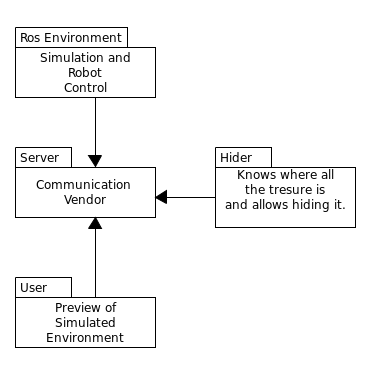
\includegraphics[width=0.7\textwidth]{figures/mainCommunication.png}
            \caption{Outline of the top level of communication.}
        \end{figure}

      With this main outline of communication done, it is also important to show how communication will be handled before it reaches a server. To do this the next two sections will talk about how communication is done in and out of ROS as well as how communication works in and out of the GUI.

      \subsubsection{Robot Operating system communication}
        ROS uses a published/subscriber\cite{publisher} mode of communication for its transfer of information. This means that while it is extremely simple to communicate between inside nodes, a new node will have to be developed that opens communication to ROS from outside sources. This can be viewed in the following figure:

          \begin{figure}[!ht]  
            \centering
              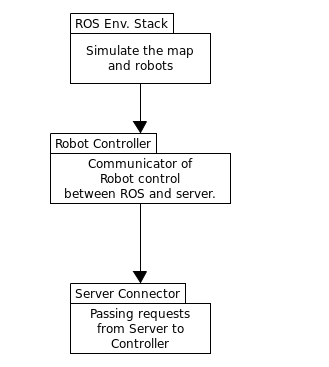
\includegraphics[width=0.8\textwidth]{figures/RosCommunication.png}
              \caption{Outline of the top level of communication.}
          \end{figure}

        The graph above presents a figure that shows that the communication starts at ROS Environment Stack. This has to be switched on for further channels to make use of the stack. Then a robot controller node has to be created to ensure that sending goals is feasible when a command comes in but it shouldn't have direct connection to the server. The report has taken advantage of publisher/subscriber mode of communication and makes the server controller and robot controller contact in that exact manner. This actually allows for modularity between nodes as neither has to be switched on first and they can be changed and modified freely per users need. Considering that ROS codebase is done either in C++ or Python, with C++ proposing a better API in ROS environment, both nodes will be created using C++ and ran inside the same package that the simulation environment runs in to ensure maximum compatibility. This gives a good of idea of how the communication will be handled inside ROS. The next section will discuss how this communication is handled inside the Graphical User Interface environment.

      \subsubsection{Graphical User Interface/Hider Communication}
        In the Graphical User Interface, we can't take advantage of the Publisher/Subscriber approach that ROS loves to use. This means that while we can easily create both the user interface and the client that connects to the server. We need to think about how communication between the two will work to ensure that both writing and listening to the server is allowed and fires events based on responses. The same can be said for the Hider interface. This Hider interface could be implemented on the ROS environment stack alongside everything else but for the sake of modularity, the report will keep it outside. To develop this environment the following proposition is made for the environment:

        \begin{figure}[!ht]  
            \centering
              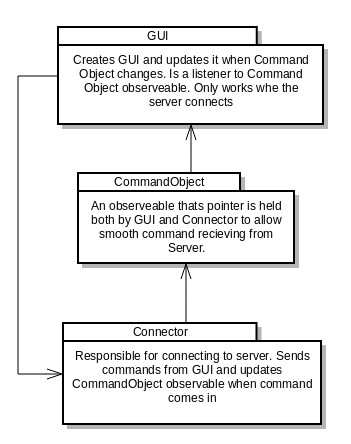
\includegraphics[width=0.8\textwidth]{figures/GUICommunication.png}
              \caption{Outline of communication inside GUI.}
          \end{figure}

        The Graphical user interface will implement an Observer design pattern to synchronize the communication between the GUI and the connector when a message comes in. The connector receives a command, changes the CommandObject and because the CommandObject was changes, the GUI as a listener will be fired and update the map. On the other side when the GUI wants to send a command, since it implements the Connector as a connection class, it should simply be able to pass the parameters directly into a command inside the Connector leaving the CommandObject strictly to the GUI to be fired when changed. With this, the report now has the design for the main protocol of communication and the next sections discuss the choices for design inside the ROS environment and GUI for the user.

    \section{ROS Environment}
      The most important consideration in design is scalability with which the simulations can run. In ROS we have two options for running the simulations one of which is Gazebo and the other Rviz for simulation preview. This is important to understand how the environment works and also if it actually works properly in terms of multi-robot environment.

      Each environment provides a certain ease of use inside the project with Gazebo allowing to build packages for robots making it a nice candidate for quick setup but also requires to constantly run Gazebo in the background which doesn't make it an ideal candidate for saving resources and performance which in the future might affect scalability. To avoid this issue, a better option would be to run Navigation Stack which is what will simulate the topics and the robot environment and to run Rviz for debugging purposes.

        \begin{figure}[!ht]  
          \centering
            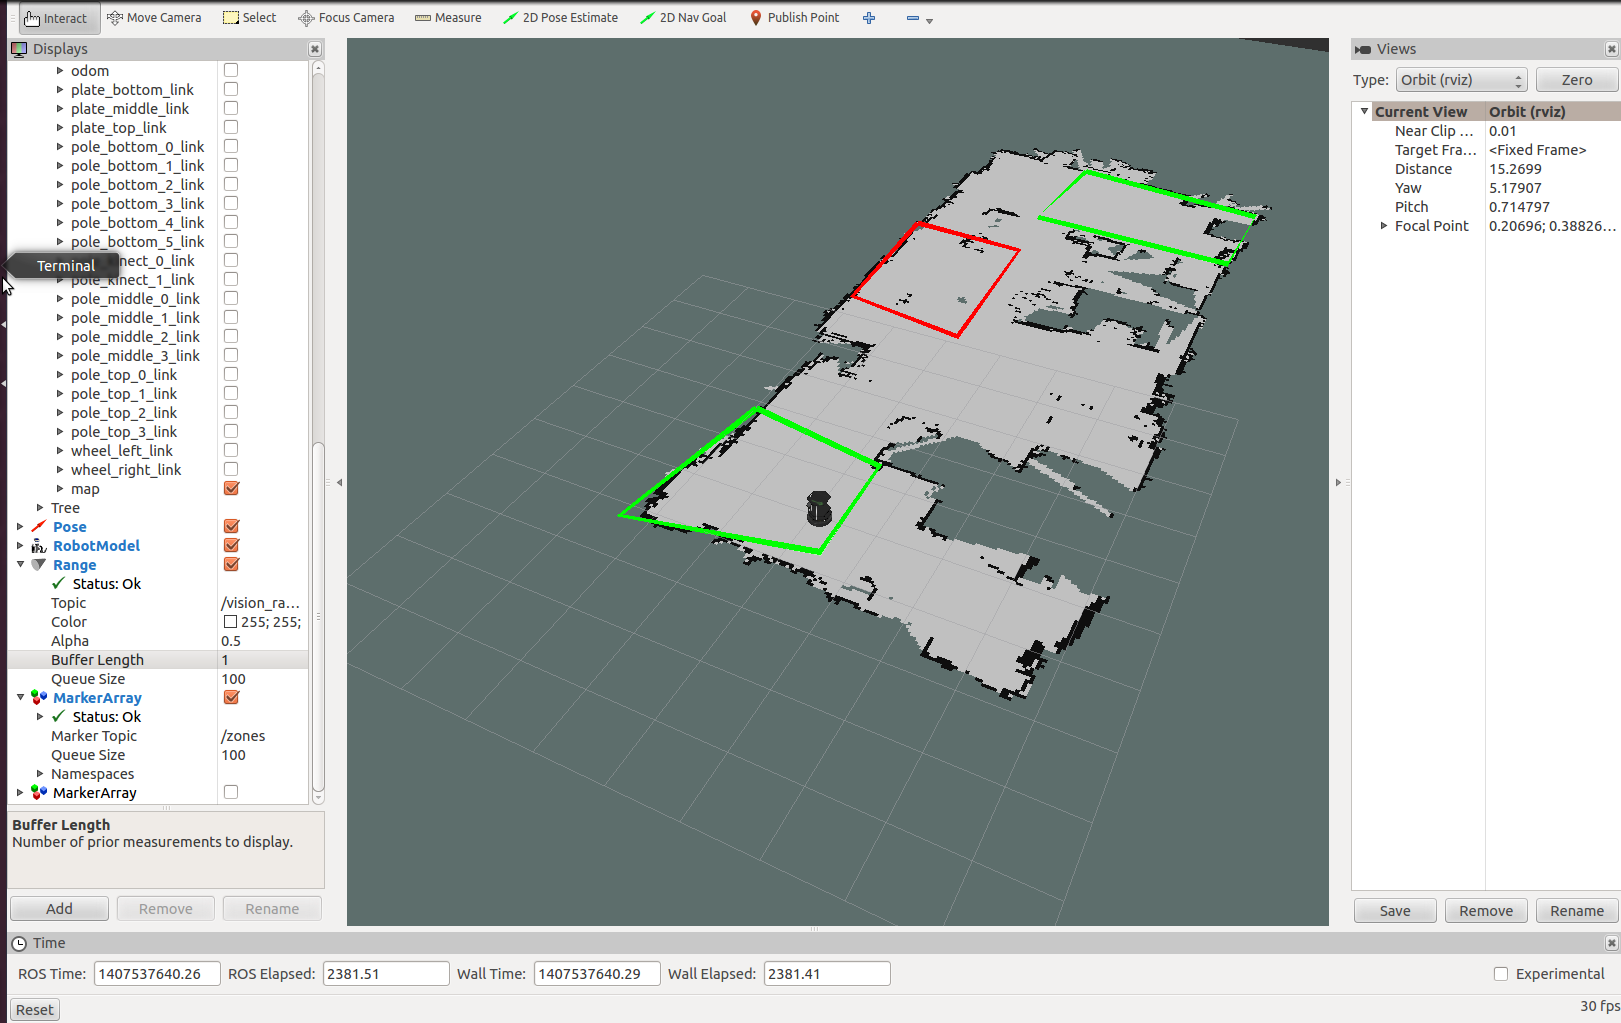
\includegraphics[width=0.6\textwidth]{figures/RVIZ.png}
            \caption{Example of Rviz running.}
        \end{figure}

      From current research, Rviz does not provide functionality in terms of displaying multiple robots but running it is optional in terms of environment so in that choice, Rviz is chosen to be the main simulation display in the first stages of the project. It will be used that when goals are set by the controller, the robot walks towards a certain path as well as ensure that the multiple layer design that ROS needs to implement in the navigation stack is chosen.

      To actually create multiple robot environment is a question of implementation and trial and error in the environment rather than design as the ROS navigation stack at this point is generally very unfamiliar however using answers provided in \cite{wiki1} we can imply that the design of the robot architecture will be as follows:

        \begin{figure}[!ht]  
          \centering
            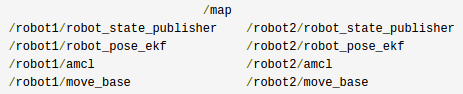
\includegraphics[width=1\textwidth]{figures/ROSPlan.png}
            \caption{Ideally how multi robot is going to work.}
        \end{figure}

      Figure above shows how two robots are mapped to the same map. The main challenge with this will be figuring out how to implement this in the Navigation stack without using gazebo for the backbone to avoid the need to consume extra resources through gazebo.

      It is important to note that originally the implementation will try to set up an environment with one robot that runs and allows to set up the GUI first. If however this doesn't pose too many issues, a two robot environment will be developed before the GUI is taken into consideration.

    \section{GUI for User and Hider}
      The GUI is the front of what the user sees and experiences through the use of application. This will be the main product that researchers will show to the users to later enquire about the dialogue model. It is therefore essential to ensure that the design is as simplistic and as intuitive as possible. After all the user should not feel like the design of the interface is in any way overwhelming. This could lead to not paying attention to the dialogue systems as well as bring on an experience that would otherwise compromise the flow of actions that lead the user from beginning to the end.

      While the previous section included an explanation of how the environment communicates with the server it did very little in explaining how the GUI is going to look or what programming language is going to be implemented to ensure both a pleasant experience for the user but also maximize compatibility with the Java Server that runs in the background and allows communication to the ROS environment. Both of these are discussed in the following sections.

      \subsubsection{The looks of the design}
        The application boasts quite a lot of information that the user needs to take in. The short list below summarizes most of the information that the user will see:
        \begin{itemize}
          \item The map and robots location on the map.
          \item List of possible robots that the user can select from
          \item Objectives of the game
          \item List of rooms that the robot can go to.
          \item Information about energy levels of various robots; each different.
          \item Dialogue windows popping up to start communication between robot and human.
        \end{itemize}

        With this list, a design can definitely start forming into shape with the last point being one of the most important ones. That the dialogues pop up rather than be placed in a sidebar or a top bar or anywhere else. The user should have a strong level of interaction with the robot as well as be able to make note of the communication that occurs. Once a robot gets a command it should communicate with the Human and notify them of possibilities or try to persuade them to do other things like go to another room or pickup a treasure that is distinct enough to others that it will be better to grab it rather than take a picture of the item if the user decides to take a picture of a distinct object.

          \begin{figure}[!ht]  
            \centering
              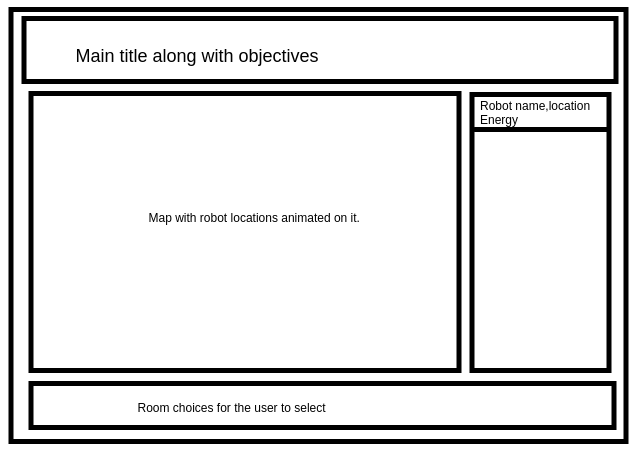
\includegraphics[width=1\textwidth]{figures/GUIDesign.png}
              \caption{Basic idea of the GUI design for the user.}
          \end{figure}

        This design largely represents the work flow of the application with the Dialogue window popping up requesting user input right in the middle of the frame to ensure that the user gives input to the robot and maximize the efficiency of the application.

        With regards to the hider GUI, it could be implemented as a GUI but creating a simple code that holds variables would make more sense as it will actually be faster to edit those than to do so through the use of GUI. It will keep external files to the minimum not requiring to run separate external files along with that .jar compiled file and with that rationale. At this point in the project it will suffice to have the Hider work at source code and change the variables inside it, compile and run accordingly.

      \subsubsection{Programming language choice}
        To develop the GUI itself, there are numerous options to choose from. Different languages offer different options and a list of possible programming languages taken under consideration in this report is:
        
          \begin{itemize}
            \item C++
            \item JavaScript
            \item Python
            \item Java
          \end{itemize}

        Each of these languages would be a good choice but to outline the main differences, each following chapter will discuss their positives and negatives.

        C++ is a great programming language for memory management and as such maximizing efficiency of the software through the use of pointers and memory dumping whenever any information is not necessary. With that, a graphical user interface could be set up in such a way that the user could execute a program and run it very easily. It does however bring a need to compile to specific operating systems like Linux, Windows or Mac depending on the platform that the software runs on\cite{cplus}. Also C++ has commands that are specific to each operating system meaning that while creating a C++ could potentially bring out the best performance, it would also create platform dependent binaries or even so, make code that is platform dependent and with that, it could potentially minimize the target audience for the project. Keeping the project as open platform as possible so that any user could run the GUI is also a very important aspect of the project.

        With JavaScript, the GUI would experience a very good boost in terms of GUI looks. Combining JavaScript with HTML could produce a very neat looking design that could update itself based on server output however the big issue with JavaScript is that it doesn't really support connecting to the server unless external platforms like socket.io\cite{socketio} are brought in. Otherwise JavaScript is AJAX dependent which means that it would either require an additional library importing and learning a new platform or, expanding the server to allow API calls but these kinds of implementations fall outside of the scope of possibility for this project.

        Python offers great ease of use, is a relatively fast language in comparison to the previously mentioned languages. It also works great with sprites and drawing GUI’s which could prove extremely useful in this project. This can be witnessed in books that teach Python programming and use sprite and GUI design as their main chapters\cite{python}. With python however, there is still an issue that was present with C++. While Python is an interpreted language, it works only if the interpreter is installed on the computer. With Linux based systems that is not an issue at all because Linux runs a lot of its software using Python so the interpreter is always pre-installed but when it comes to Windows, this interpreter is not installed as Windows tends to keep to its .exe file system and that again, would limit the scope for the audience.

        Java is the language that the Server was developed in. It is a language that has pre-built GUI libraries called Swing and AWT which allows for a fast GUI prototype implementation and is even use for general development in bigger corporations. These two are definitely favorable when it comes to the GUI created in this project. Java is also present on most PC’s because while systems don't use it as a pre-requisite, a lot of software is implemented using Java and there is a very high chance that any computer visited will have Java working on it. This provides a rationale for choosing Java for the implementation of the GUI.

    \section{Testing design}
      This project will taken upon itself a test driven development sprint where a set of criteria outlined in the specification will guide the way towards a successful implementation of the product. It is however important to outline some criteria other than the simplistic ones that are given in the specification for clarity purposes.

      One of these is to outline a use case for when the users are using the GUI to give an outline of what a successful implementation should do. With this user case, testing will later be carried out to ensure that the application has successfully undergone implementation purposes. Figure 4.7 demonstrates the basic use case that outlines the what the user should be able to do inside the application.

        \begin{figure}[!ht]  
          \centering
            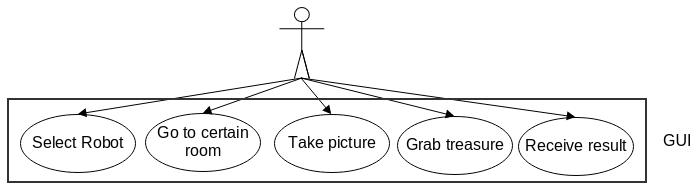
\includegraphics[width=1\textwidth]{figures/GuiUseCase2.png}
            \caption{Use Case for GUI.}
        \end{figure}

      With this we can see all the commands that are available to the user all of which should run successfully and without any issues.For a better explanation of the stages through which the application should go, a flow chart needs to be constructed. Such a flowchart will provide a better explanation of how the system works and in which areas lies logic that needs to be tested. Diagram presented in Figure 4.8 demonstrates the extent to which each logic function will need to be tested.

        \begin{figure}[!ht]  
          \centering
            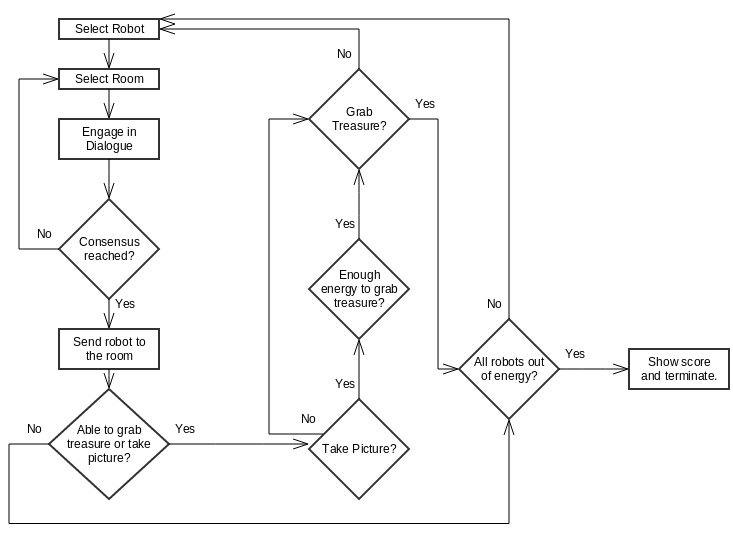
\includegraphics[width=1.1\textwidth]{figures/flowChart.png}
            \caption{Flow chart for GUI use.}
        \end{figure}

      It can be then implied that for the test driven implemented in this project, the application will need to reach the terminate state while ensuring that each decision in the use case has been tested. This will provide enough information to say that the product was fully finished along with the information provided in the specification.